\documentclass[dvipdfmx]{jsarticle}
\usepackage[dvipdfmx]{graphicx}
\usepackage{amsmath, amssymb}
\usepackage{mathtools}
\usepackage{here}
\begin{document}
\title{週間進捗報告}
\author{権藤陸}
\maketitle
\section{進捗}
\begin{itemize}
    \item 取得済みのFMCWレーダデータと,FMCWレーダ(T14 2D)の場所確認
    \item T14 2Dのマニュアルの確認
    \item 遠藤さんにいただいたコードの実行・確認
\end{itemize}
\section{レンジアングルマップ}
サンプルコードを実行し,レンジアングルマップを表示した.
壁までの距離6m,設定は以下の通り.
\begin{figure}[htbp]
\begin{center}
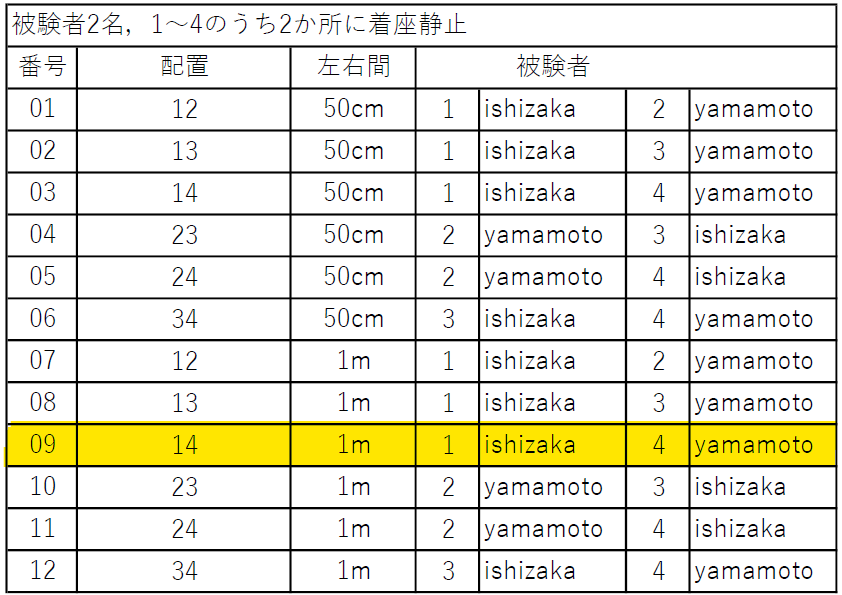
\includegraphics[width=0.6\linewidth]{./img/setting.png}
\end{center}
\caption{実験諸元}
\end{figure}

\begin{figure}[H]
\begin{center}
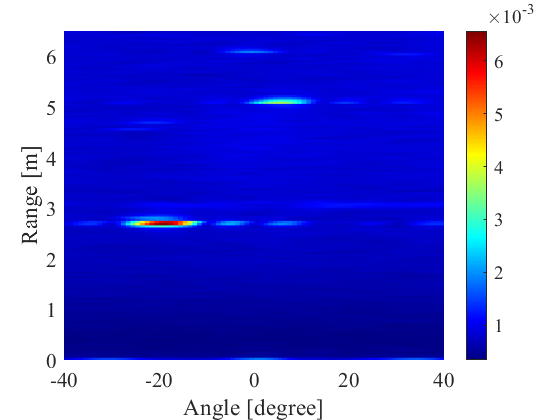
\includegraphics[width=0.8\linewidth]{./img/range_doppler_sample.png}
\end{center}
\caption{レンジアングルマップ}
\end{figure}

\begin{figure}[H]
\begin{center}
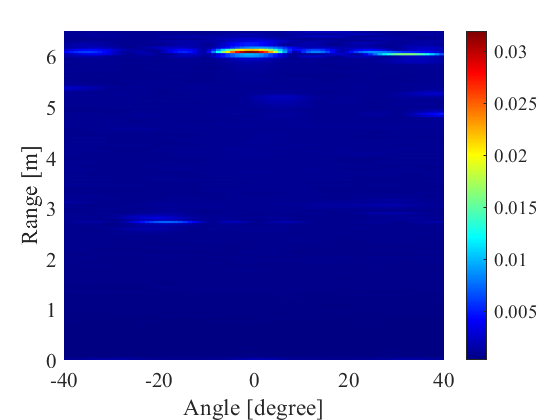
\includegraphics[width=0.8\linewidth]{./img/range_doppler_sample2.png}
\end{center}
\caption{レンジアングルマップ(信号強度の閾値とレンジ変更)}
\end{figure}
\section{計画}
\begin{itemize}
    \item いただいたコードを確認し,書き直す
    \item 実験について検討する
\end{itemize}

\end{document}